\documentclass{rapidsart}

\volume{0}
\issue{0}
\pubmonth{Juli}
\pubyear{2026}
\articletype{research-article}
\doi{0000}
\firstpage{1}
\lastpage{13}

\theoremstyle{plain}
\newtheorem{thm}{Theorem}
\newtheorem{lemma}{Lemma}

\theoremstyle{remark}
\newtheorem{remark}{Remark}
\theoremstyle{definition}
\newtheorem{defin}{Definition}
\hyphenation{de-si-de-rium}
\renewcommand{\thesection}{\arabic{section}}

\usepackage{multirow}
\usepackage{indentfirst}
\usepackage{float}
\usepackage{enumitem}
\usepackage[indonesian]{babel}
\usepackage{natbib}
\usepackage{graphicx}
\usepackage{tikz}
\usepackage{adjustbox}
\usepackage{booktabs}
\usepackage{amsmath}
\usepackage{amsfonts}
\usepackage{longtable,array}
\usetikzlibrary{shapes.geometric, shapes.symbols, arrows.meta, positioning, calc, fit, backgrounds, shapes.multipart}

\tikzset{
    startstop/.style={rectangle, rounded corners=5pt, minimum width=1.8cm, minimum height=0.6cm, text centered, draw=black, line width=0.6pt, fill=green!20, font=\scriptsize\bfseries},
    process/.style={rectangle, minimum width=1.8cm, minimum height=0.6cm, text centered, draw=black, line width=0.6pt, fill=blue!12, font=\scriptsize},
    predefined/.style={rectangle, minimum width=1.8cm, minimum height=0.6cm, text centered, draw=black, line width=0.6pt, fill=orange!20, font=\scriptsize, 
        path picture={\draw[line width=0.5pt] ([xshift=2.5pt]path picture bounding box.north west) -- ([xshift=2.5pt]path picture bounding box.south west);
        \draw[line width=0.5pt] ([xshift=-2.5pt]path picture bounding box.north east) -- ([xshift=-2.5pt]path picture bounding box.south east);}},
    data/.style={trapezium, trapezium left angle=70, trapezium right angle=110, minimum width=1.6cm, minimum height=0.5cm, text centered, draw=black, line width=0.6pt, fill=yellow!20, font=\scriptsize},
    database/.style={cylinder, shape border rotate=90, draw=black, line width=0.6pt, minimum height=0.7cm, minimum width=1.1cm, fill=purple!15, font=\tiny, aspect=0.3},
    decision/.style={diamond, minimum width=1.4cm, minimum height=1cm, text centered, draw=black, line width=0.6pt, fill=red!12, font=\tiny, inner sep=0pt, aspect=2},
    onpage/.style={circle, minimum size=0.45cm, draw=black, line width=0.6pt, fill=white, font=\tiny\bfseries},
    offpage/.style={signal, signal to=south, minimum width=0.5cm, minimum height=0.45cm, draw=black, line width=0.6pt, fill=gray!15, font=\tiny\bfseries},
    arrow/.style={thick, -Stealth, line width=0.5pt},
    subbox/.style={draw=orange!70!black, line width=0.8pt, rounded corners=2pt, fill=orange!5, inner sep=4pt}
}

\begin{document}

\begin{frontmatter}

    \title{Rancang Bangun Pipeline ETL Multi-Sumber untuk Integrasi Data Profil dan Publikasi Ilmiah Dosen Berbasis Apache Airflow}
    \runtitle{Rancang Bangun Pipeline ETL Data Akademik Berbasis Airflow}

    \author{\inits{R.Y.}\fnms{Rizky Yanuar} \snm{Kristianto}
        \thanksref{c1}
        \ead{rizky.22017@mhs.unesa.ac.id}}

    \author{\inits{I.F.}\fnms{Ibnu Febry} \snm{Kurniawan}}

    \author{\inits{H.A.}\fnms{Hasanuddin} \snm{Al-Habib}}

    \thankstext[type=corresp,id=c1]{Corresponding author.}

    \address{
        \institution{Program Studi S1 Sains Data, Fakultas Matematika dan Ilmu Pengetahuan Alam, Universitas Negeri Surabaya},
        \cny{Indonesia}
    }

    \begin{abstrak}
        Integrasi data akademik di perguruan tinggi sering kali terhambat oleh fragmentasi dan heterogenitas data yang tersebar di berbagai platform internal dan eksternal. Penelitian ini bertujuan untuk merancang dan mengimplementasikan pipeline \textit{Extract, Transform, Load} (ETL) otomatis berbasis kontainer untuk menyelaraskan data profil dosen dan rekam jejak publikasi ilmiah pada rumpun Informatika dan Komputer Universitas Negeri Surabaya. Sistem yang dikembangkan menggunakan \textit{Apache Airflow} sebagai orkestrator alur kerja yang di-\textit{deploy} pada infrastruktur awan AWS EC2 menggunakan Docker Compose. Tahap \textit{Extract} menarik data dari enam sumber heterogen, yaitu PDDIKTI, SIAKADU, SimCV, Sinta, Elsevier Scopus, dan Google Scholar. Tahap \textit{Transform} melakukan pembersihan gelar akademik, penggabungan cerdas (\textit{smart merge}) berbasis \texttt{SequenceMatcher} untuk resolusi identitas dosen, serta pengeliminasian duplikasi publikasi multi-indeksasi menggunakan \textit{deterministic hashing} berbasis MD5. Tahap \textit{Load} melakukan pemuatan dan sinkronisasi data relasional ke basis data PostgreSQL. Hasil penelitian menunjukkan bahwa pipeline ETL berhasil mengakuisisi data dari 128 dosen aktif dan 7.889 rekaman publikasi mentah, serta melebur 864 artikel duplikat menjadi 6.161 publikasi unik. Selain itu, penerapan rotasi proxy residensial BrightData dan mekanisme \textit{checkpoint recovery} berhasil mengamankan proses scraping dari pemblokiran IP serta menghemat kuota API eksternal hingga 85\%. Rancang bangun ini memberikan fondasi repositori akademik yang terintegrasi, konsisten, dan terbaharui secara otomatis bagi institusi.
    \end{abstrak}

    \begin{kunciwords}
        \kwd{Pipeline ETL}
        \kwd{Apache Airflow}
        \kwd{Integrasi Data}
        \kwd{Web Scraping}
        \kwd{Publikasi Dosen}
    \end{kunciwords}

    \begin{abstract}
        Academic data integration in higher education institutions is frequently hindered by data fragmentation and heterogeneity across disparate internal systems and external indexing platforms. This study aims to design and implement an automated, containerized Extract, Transform, Load (ETL) pipeline to harmonize faculty profiles and scientific publication records within the Computer Science and Informatics department at the State University of Surabaya. The proposed system utilizes \textit{Apache Airflow} as a workflow orchestrator deployed on an AWS EC2 cloud infrastructure using Docker Compose. The Extract phase parallelly retrieves data from six heterogeneous sources: PDDIKTI, SIAKADU, SimCV, Sinta, Elsevier Scopus, and Google Scholar. The Transform phase executes academic title normalization, \texttt{SequenceMatcher}-based smart merging for faculty identity resolution, and MD5 deterministic hashing to eliminate multi-indexed publication duplicates. Finally, the Load phase synchronizes relational data models into PostgreSQL. Empirical evaluation demonstrates that the ETL pipeline successfully acquired profiles of 128 active faculty members and 7,889 raw publication records, consolidating 864 overlapping articles into 6,161 unique publications. Furthermore, BrightData residential proxy rotation and checkpoint recovery mechanisms effectively mitigate IP blocking and conserve up to 85\% of external API quotas. This architecture provides a robust, scalable, and automated repository foundation for institutional academic intelligence.
    \end{abstract}

    \begin{keywords}
        \kwd{ETL Pipeline}
        \kwd{Apache Airflow}
        \kwd{Data Integration}
        \kwd{Web Scraping}
        \kwd{Lecturer Publication}
    \end{keywords}

    \received{\today}
    \revised{\today}
    \accepted{\today}

\end{frontmatter}

\section{Pendahuluan}
\begin{sloppypar}
    Berkembangnya teknologi dan informasi saat ini berlangsung sangat pesat sehingga menghasilkan akumulasi data berukuran masif. Kumpulan data tersebut perlu dikelola dalam suatu \textit{Database Management System} (DBMS) yang terstruktur untuk menghasilkan kebutuhan informasi yang cepat, akurat, dan bernilai strategis. Pada lingkungan pendidikan tinggi, teknologi informasi mendukung berbagai aktivitas esensial, seperti penilaian kinerja publikasi dosen dan pelaporan capaian akademik institusi. Namun, \cite{setiawan2022pddikti} menyatakan bahwa pertumbuhan volume data ilmiah yang masif menghadirkan tantangan tata kelola yang kompleks akibat fragmentasi data di berbagai platform eksternal maupun internal. Studi pembandingan cakupan basis data ilmiah menunjukkan bahwa tidak ada satu pun portal pengindeks tunggal yang mampu mencakup seluruh karya ilmiah secara komprehensif, sehingga pengintegrasian multi-sumber seperti Scopus, Google Scholar, dan basis data nasional menjadi sangat krusial \citep{visser2021comparison, MartínMartín2021}. Pada Universitas Negeri Surabaya (UNESA), data profil dosen di sistem internal seperti SIAKADU dan SimCV belum terhubung secara otomatis dengan pangkalan data nasional PDDIKTI maupun indeksasi publikasi global, sehingga menghambat integrasi informasi profil dosen secara \textit{real-time}.

    Untuk menyatukan dan menyajikan data akademik tersebut secara terstruktur, penerapan \textit{data warehouse} menjadi repositori data terpusat yang sangat penting. Agar data dari berbagai platform eksternal dan internal dapat diselaraskan secara konsisten, diperlukan arsitektur \textit{data pipeline} yang andal untuk mengalirkan data dari sistem sumber ke media penyimpanan terpusat. Dalam lingkungan berbasis data modern, \textit{data pipeline} memfasilitasi perpindahan data dari berbagai sumber ke sistem tujuan melalui alur kerja \textit{Extract, Transform, and Load} (ETL) yang mencakup pengambilan data, pembersihan, pengayaan, hingga pemuatan ke \textit{data warehouse} \citep{shojaeegrad2024data}. Selain itu, tantangan utama pada integrasi data akademik heterogen terletak pada ambiguitas penulisan nama dosen dan tumpang tindih (*overlap*) rekaman publikasi antar-platform, yang membutuhkan teknik resolusi identitas dan deduplikasi data secara otomatis \citep{tekles2020author}.

    Penelitian terdahulu mengenai penerapan \textit{data warehouse} di perguruan tinggi oleh \cite{oslan2018proses} telah menerapkan ETL untuk profil mahasiswa. Namun, proses ETL dan pembersihan data pada penelitian tersebut masih dilakukan secara manual tanpa sistem orkestrasi yang fleksibel. Sementara itu, otomatisasi dan orkestrasi alur kerja ETL menggunakan platform seperti Apache Airflow terbukti dapat meningkatkan stabilitas dan efisiensi pemrosesan data skala besar secara terjadwal \citep{koppula2020etl}.

    Untuk mengatasi keterbatasan tersebut, penelitian ini merancang dan mengimplementasikan pipeline ETL otomatis berbasis Apache Airflow yang di-deploy pada infrastruktur awan AWS EC2. Sistem ini mengintegrasikan data profil dosen dan publikasi ilmiah dari enam sumber heterogen (PDDIKTI, SIAKADU, SimCV, Sinta, Scopus, dan Google Scholar) dengan menerapkan *smart merge* dan rotasi proxy resilien. Rancang bangun ini diharapkan dapat memberikan fondasi repositori akademik terintegrasi, konsisten, dan terbaharui secara otomatis bagi institusi.
\end{sloppypar}

\section{Metode}
\begin{sloppypar}

    \subsection{Alur Penelitian}
    Tahapan pelaksanaan penelitian ini diawali dengan mengidentifikasi sumber data dan merancang arsitektur sistem ETL, dilanjutkan dengan pengembangan konektor ekstraksi, implementasi transformasi (pembersihan, smart merge, standarisasi kata kunci), penyusunan mekanisme load, serta pengujian resiliensi pipeline menggunakan orkestrasi Apache Airflow. Alur penelitian selengkapnya digambarkan pada Gambar~\ref{fig:alur-penelitian}.

    \begin{figure}[htbp]
        \centering
        \definecolor{researchblue}{HTML}{005086}
        \begin{adjustbox}{max width=\textwidth, center}
            \begin{tikzpicture}[
                    block/.style={
                            rectangle,
                            fill=researchblue,
                            text=white,
                            minimum width=3.8cm,
                            minimum height=2.2cm,
                            align=center,
                            font=\small\bfseries,
                            inner sep=8pt
                        },
                    arrow/.style={
                            line width=2.5pt,
                                -{Stealth[scale=1.2]},
                            draw=researchblue,
                            shorten >=6pt,
                            shorten <=6pt
                        }
                ]
                \node (n1) [block] at (0, 0) {Identification\\\& Needs\\Analysis};
                \node (n2) [block] at (5.0, 0) {ETL Pipeline\\Architecture\\Design};
                \node (n3) [block] at (10.0, 0) {Implementation of\\ETL Pipeline and\\Data Warehouse};
                \node (n4) [block] at (15.0, 0) {ETL Pipeline\\Testing};

                \draw [arrow] (n1) -- (n2);
                \draw [arrow] (n2) -- (n3);
                \draw [arrow] (n3) -- (n4);
            \end{tikzpicture}
        \end{adjustbox}
        \caption{Alur Penelitian}
        \label{fig:alur-penelitian}
    \end{figure}

    \subsection{Identifikasi dan Analisis Kebutuhan subject data}
    Identifikasi kebutuhan informasi eksekutif dilakukan menggunakan pendekatan strategi penelusuran informasi-informasi yang biasa dilaporkan oleh pimpinan program studi dan fakultas. Sumber acuan format laporan eksekutif tersebut berasal dari instrumen borang akreditasi program studi (seperti kriteria kinerja dosen oleh BAN-PT atau Lembaga Akreditasi Mandiri), kuesioner Audit Mutu Akademik Internal (AMAI) universitas, laporan evaluasi diri institusi, serta kebutuhan pemetaan kepakaran riset dosen. Kebutuhan utama yang diidentifikasi meliputi pelaporan berkala mengenai produktivitas publikasi ilmiah dosen, rekam jejak indeksasi global (seperti sitasi dan \textit{h-index}), serta klasifikasi klaster keahlian berdasarkan kata kunci riset.

    Langkah selanjutnya adalah melakukan pemetaan antara sumber acuan format dengan sumber data akademik yang telah tersedia. Sistem yang dikembangkan dalam penelitian ini memetakan kebutuhan data dari pangkalan data internal kampus seperti Web setiap prodi dan SimCV serta platform pengindeksan seperti PDDIKTI, Sinta, Scopus, dan Google Scholar. Hasil analisis kebutuhan data dan informasi sistem yang akan dikembangkan disusun dan dikelompokkan berdasarkan subjek utama \textit{data warehouse} akademik dosen, yaitu Profil Dosen dan Publikasi Ilmiah. Penentuan subjek ini didasarkan pada aktivitas riset dosen rumpun Informatika dan Komputer (Infokom) UNESA, atribut yang akan di pakai seperti dirangkum pada Tabel~\ref{tab:deskripsi-dataset}.

    \begingroup
    \small
    \renewcommand{\arraystretch}{1.2}
    \begin{longtable}{ll>{\raggedright\arraybackslash}p{0.40\textwidth}>{\raggedright\arraybackslash}p{0.18\textwidth}}
        \caption{Hasil Analisis Kebutuhan Data} \label{tab:deskripsi-dataset}                                                                                            \\
        \toprule
        \textbf{Kategori Data} & \textbf{Nama Atribut}   & \textbf{Jenis Informasi}                                                         & \textbf{Sumber Data}       \\
        \midrule
        \endfirsthead
        \caption[]{Hasil Analisis Kebutuhan Data (Lanjutan)}                                                                                                             \\
        \toprule
        \textbf{Kategori Data} & \textbf{Nama Atribut}   & \textbf{Jenis Informasi}                                                         & \textbf{Sumber Data}       \\
        \midrule
        \endhead
        \midrule
        \multicolumn{4}{r}{\textit{Bersambung ke halaman berikutnya...}}                                                                                                 \\
        \endfoot
        \bottomrule
        \endlastfoot
        Profil Dosen           & \texttt{nama\_dosen}    & Nama lengkap dosen beserta gelar akademik yang telah diverifikasi                & SIAKADU, SimCV, PDDIKTI    \\
                               & \texttt{nip}            & Nomor Induk Pegawai sebagai identitas administratif dosen                        & SIAKADU, SimCV, PDDIKTI    \\
                               & \texttt{nidn}           & Nomor Induk Dosen Nasional sebagai identitas dosen pada pangkalan data nasional  & PDDIKTI                    \\
                               & \texttt{prodi}          & Program studi tempat dosen berafiliasi                                           & SIAKADU, SimCV, PDDIKTI    \\
                               & \texttt{scholar\_id}    & ID profil \textit{Google Scholar} untuk menghubungkan dosen dengan publikasi     & Web prodi, Sinta           \\
                               & \texttt{scopus\_id}     & ID profil \textit{Scopus} untuk menelusuri rekam publikasi terindeks             & Web prodi, Sinta           \\
                               & \texttt{sinta\_id}      & ID profil SINTA untuk pelacakan kinerja akademik dosen                           & Web prodi, Sinta           \\
        \midrule
        Publikasi Ilmiah       & \texttt{authors}        & Daftar penulis yang berkontribusi dalam artikel ilmiah                           & Scopus, Google Scholar     \\
                               & \texttt{title}          & Judul publikasi ilmiah sebagai representasi utama dokumen                        & Scopus, Google Scholar     \\
                               & \texttt{year}           & Tahun publikasi untuk mendukung pencarian dan analisis temporal                  & Scopus, Google Scholar     \\
                               & \texttt{journal}        & Nama jurnal, konferensi, atau prosiding tempat publikasi diterbitkan             & Scopus, Google Scholar     \\
                               & \texttt{link}           & Tautan menuju halaman penerbit, repositori, atau dokumen PDF                     & Scopus, Google Scholar     \\
                               & \texttt{abstract}       & Abstrak artikel ilmiah sebagai sumber informasi untuk sistem manajemen publikasi & Scopus, Google Scholar     \\
                               & \texttt{keywords}       & Kata kunci publikasi ilmiah untuk kategorisasi topik penelitian                  & Scopus, Google Scholar     \\
                               & \texttt{document\_type} & Jenis publikasi seperti \textit{Article} atau \textit{Conference Paper}          & Scopus, Google Scholar     \\
                               & \texttt{doi}            & \textit{Digital Object Identifier} sebagai identitas digital unik publikasi      & Scopus, Google Scholar     \\
                               & \texttt{tldr}           & Intisari singkat artikel ilmiah untuk kemudahan penelusuran data publikasi       & OpenAlex, Semantic Scholar \\
    \end{longtable}
    \endgroup

    \subsection{Perancangan Proses ETL}
    Perancangan proses ETL (\textit{Extract, Transform, Load}) bertujuan untuk merumuskan logika pemindahan dan pemetaan data dari sumber data mentah (\textit{source}) ke dalam basis data target, serta merancang ketergantungan tugas (\textit{task dependency}) di dalam \textit{Directed Acyclic Graph} (DAG) Airflow. Perancangan ini menjamin bahwa seluruh data dosen dan karya ilmiahnya dapat diintegrasikan dengan konsistensi relasional tanpa mengalami kegagalan proses di tengah jalan. Detail rancangan logika arsitektur proses ETL disajikan pada Gambar~\ref{fig:rancangan-logika-etl}.

    \begin{figure}[htbp]
        \centering
        \begin{adjustbox}{max width=0.95\textwidth, center}
            \begin{tikzpicture}[scale=0.9, transform shape,
                    container/.style={draw=black, rounded corners=8pt, minimum height=6.2cm, align=center, line width=0.6pt},
                    db/.style={cylinder, shape border rotate=90, draw=black, minimum height=1.1cm, minimum width=1.6cm, fill=white, font=\tiny, align=center, aspect=0.25, text width=1.5cm},
                    predefined/.style={rectangle, draw=black, minimum width=2.1cm, minimum height=0.8cm, text width=1.9cm, text centered, font=\tiny\bfseries, align=center, fill=white,
                            path picture={
                                    \draw[line width=0.5pt] ([xshift=2.5pt]path picture bounding box.north west) -- ([xshift=2.5pt]path picture bounding box.south west);
                                    \draw[line width=0.5pt] ([xshift=-2.5pt]path picture bounding box.north east) -- ([xshift=-2.5pt]path picture bounding box.south east);
                                }
                        },
                    decision/.style={diamond, draw=black, minimum width=1.6cm, minimum height=0.9cm, text width=1.3cm, text centered, font=\tiny\bfseries, align=center, fill=white, aspect=1.8, inner sep=0.5pt},
                    arrow/.style={thick, -Stealth, line width=0.6pt}
                ]

                % Background Containers
                \node (sumber_box) [container, fill=blue!10, text width=2.4cm, minimum width=2.6cm] at (-0.3, 0) {};
                \node (staging_box) [container, fill=green!12, text width=8.6cm, minimum width=9.2cm] at (6.6, 0) {};
                \node (penyimpanan_box) [container, fill=purple!10, text width=2.4cm, minimum width=2.6cm] at (13.5, 0) {};

                % Labels for Containers (at the bottom)
                \node[font=\tiny\bfseries] at (-0.3, -2.7) {SUMBER DATA};
                \node[font=\tiny\bfseries] at (6.6, -2.7) {DATA STAGING};
                \node[font=\tiny\bfseries, align=center] at (13.5, -2.7) {PENYIMPANAN \\ DATA};

                % Inside SUMBER DATA
                \node (db_internal) [db] at (-0.3, 1.8) {Data SIAKADU \\ \& SimCV};
                \node (db_pddikti) [db] at (-0.3, 0.3) {Data PDDIKTI};
                \node (db_indeks) [db] at (-0.3, -1.2) {Data Scopus \\ \& Scholar};

                % Block Arrow 1 (Sumber -> Staging)
                \draw[draw=black, fill=gray!30] (1.35, 0.2) -- (1.5, 0.2) -- (1.5, 0.1) -- (1.65, 0.3) -- (1.5, 0.5) -- (1.5, 0.4) -- (1.35, 0.4) -- cycle;

                % Inside DATA STAGING
                \node (step_link) [predefined] at (3.4, 1.2) {Membuat Koneksi \\ \& Ingest Data};
                \node (step_load) [predefined] at (3.4, -0.8) {Memuat Data \\ Mentah ke Staging};
                \node (check_data) [decision] at (6.7, -0.8) {Mengecek \\ Validitas Data};
                \node (db_staging) [db] at (6.7, 0.8) {Data Staging \\ Akademik};
                \node (step_clean) [predefined] at (9.8, 2.0) {Cleansing dan \\ Transformasi};
                \node (step_script) [predefined] at (9.8, 0.2) {Script untuk \\ Loading Data};

                % Inside DATA STAGING Arrows
                \draw [arrow] (step_link) -- (step_load);
                \draw [arrow] (step_load) -- (check_data);
                \draw [arrow] (check_data) -- node[right, font=\tiny\bfseries] {Valid} (db_staging);
                \draw [arrow] (check_data.south) -- (6.7, -1.7) -- node[above, font=\tiny\bfseries] {Tidak Valid} (3.4, -1.7) -- (step_load.south);
                \draw [arrow] (db_staging.north) |- (step_clean.west);
                \draw [arrow] (step_clean) -- (step_script);

                % Block Arrow 2 (Staging -> Penyimpanan)
                \draw[draw=black, fill=gray!30] (11.55, 0.2) -- (11.7, 0.2) -- (11.7, 0.1) -- (11.85, 0.3) -- (11.7, 0.5) -- (11.7, 0.4) -- (11.55, 0.4) -- cycle;

                % Inside PENYIMPANAN DATA
                \node (db_dw) [db] at (13.5, 0.1) {Database \\ Akademik};

            \end{tikzpicture}
        \end{adjustbox}
        \caption{Rancangan logika arsitektur proses ETL data akademik}
        \label{fig:rancangan-logika-etl}
    \end{figure}

    Secara garis besar, rancangan proses ETL pada penelitian ini dibagi menjadi tiga rancangan utama yang dirinci ke dalam sub-tahapan berikut:

    \subsubsection{Tahap Ekstraksi Data}
    Mengacu pada blok kontainer \textbf{SUMBER DATA} dan langkah awal pada area \textbf{DATA STAGING} (Gambar~\ref{fig:rancangan-logika-etl}), tahap ekstraksi diawali dengan proses \textit{"Membuat Koneksi \& Ingest Data"} serta \textit{"Memuat Data Mentah ke Staging"}. Tahap ini bertujuan untuk menarik data mentah profil dosen dan rekam jejak publikasi ilmiah dari enam sumber data eksternal dan internal secara independen:
    \begin{enumerate}
        \item \textbf{Ekstraksi Profil Dosen:} Data ditarik dari direktori dosen pada situs web program studi UNESA melalui teknik \textit{web scraping} untuk mendapatkan informasi awal berupa nama, program studi, dan halaman asal. Selanjutnya, sistem memanggil API PDDIKTI Feeder \citep{setiawan2022pddikti} untuk memverifikasi profil resmi dosen guna mengamankan atribut NIDN (Nomor Induk Dosen Nasional). Selain itu, sistem mengakses database internal SIAKADU dan SimCV untuk melengkapi Nomor Induk Pegawai (NIP) serta data kepegawaian internal kampus. Terakhir, tautan pengenal unik seperti Sinta ID dan Scholar ID diekstraksi dari direktori publikasi masing-masing dosen.
        \item \textbf{Ekstraksi Publikasi Ilmiah:} Metadata publikasi ditarik secara terstruktur menggunakan REST API Elsevier Scopus dengan memanfaatkan atribut \texttt{scopus\_id} dosen. Untuk publikasi yang terindeks di Google Scholar, ekstraksi dilakukan menggunakan \textit{crawler} khusus. Karena Google Scholar menerapkan sistem deteksi bot yang ketat, skrip crawler diintegrasikan dengan rotasi proxy residensial \textit{BrightData Web Unlocker} guna menghindari deteksi CAPTCHA dan pemblokiran alamat IP.
    \end{enumerate}
    Setiap data mentah yang berhasil ditarik kemudian melalui tahapan keputusan \textit{"Mengecek Validitas Data"} (Gambar~\ref{fig:rancangan-logika-etl}). Jika data mentah terdeteksi rusak atau gagal terunduh, alur akan mengulang pemuatan data mentah (cabang \textit{Tidak Valid}), sedangkan data mentah yang sesuai format dasar (cabang \textit{Valid}) akan disimpan ke dalam repositori \textit{"Data Staging Akademik"}. Untuk menjaga resiliensi proses ekstraksi terhadap kegagalan jaringan atau batasan laju permintaan (\textit{rate limits}), setiap tugas ekstraksi diorkestrasi menggunakan kebijakan percobaan ulang otomatis (\textit{automatic retry}) sebanyak dua kali dengan jeda waktu \textit{exponential backoff} selama lima menit.

    \subsubsection{Tahap Transformasi Data}
    Setelah data mentah tervalidasi dan tersimpan di dalam repositori \textit{"Data Staging Akademik"} (Gambar~\ref{fig:rancangan-logika-etl}), alur proses dilanjutkan ke tahap utama \textit{"Cleansing dan Transformasi"}. Tahap transformasi dalam pipeline ETL melakukan pembersihan data (\textit{cleansing}) dan penggabungan profil yang duplikat sebelum data siap dimuat ke dalam database target. Langkah-langkah transformasi data ini meliputi:
    \begin{enumerate}
        \item \textbf{Pembersihan dan Deduplikasi Data (\textit{Cleansing}):} Proses pembersihan diawali dengan normalisasi string nama dosen, di mana seluruh gelar akademik (seperti Prof., Dr., M.T., dll.) serta tanda baca non-alfabet dihapus sehingga hanya menyisakan karakter alfabet huruf kecil untuk memudahkan pencocokan identitas. Selanjutnya, sistem melakukan deduplikasi publikasi dari platform Scopus dan Google Scholar dengan menggenerasikan kunci unik deterministik (\texttt{paper\_id}) menggunakan algoritma hash MD5 32-karakter. Jika dokumen memiliki DOI valid, hash dihitung dari string \texttt{doi:\{normalized\_doi\}}. Jika DOI tidak tersedia, hash dihitung dari kombinasi judul yang dinormalisasi dan tahun publikasi: \texttt{title:\{clean\_title\}\_year:\{year\_str\}}. Dokumen dengan nilai hash yang sama dilebur (\textit{merge}) menjadi satu rekaman unik, sedangkan dokumen tanpa judul yang jelas atau tahun terbit tidak valid dieliminasi dari pipeline.
        \item \textbf{Resolusi Identitas Dosen (\textit{Smart Merge - Transformation}):}
              Setelah nama dinormalisasi, proses penggabungan dilakukan menggunakan algoritma \texttt{SequenceMatcher} \citep{christen2012data} untuk mengukur rasio kemiripan string nama:
              \begin{equation}
                  \text{Ratio}(s_1, s_2) = \frac{2 \times M}{|s_1| + |s_2|}
                  \label{eq:string-ratio}
              \end{equation}
              di mana $M$ menyatakan jumlah karakter yang cocok secara berurutan, sedangkan $|s_1|$ dan $|s_2|$ menyatakan panjang masing-masing string nama. Penggabungan profil disetujui secara otomatis jika skor kemiripan $\ge 0.95$. Jika skor berada pada rentang $0.85$ hingga $0.95$, sistem melakukan verifikasi tambahan dengan mencocokkan program studi pengampu dosen tersebut untuk menghindari salah identifikasi (\textit{false positive}) pada dosen yang memiliki kemiripan nama.
    \end{enumerate}

    \subsubsection{Tahap Pemuatan Data}
    Tahap akhir implementasi ETL dipicu oleh proses \textit{"Script untuk Loading Data"} pada area staging (Gambar~\ref{fig:rancangan-logika-etl}) untuk memindahkan data yang telah bersih dan terstruktur dari area staging ke kontainer \textbf{PENYIMPANAN DATA} yaitu \textit{"Database Akademik"} (PostgreSQL). Data relasional dimuat menggunakan operasi \textit{UPSERT} berbasis constraint Primary Key (\texttt{nip} untuk profil dosen, \texttt{paper\_id} untuk metadata publikasi, dan composite key \texttt{(paper\_id, nip)} untuk relasi kepengarangan). Pendekatan ini menjamin sifat \textit{idempotensi}, di mana eksekusi ulang pipeline ETL tidak akan menduplikasi rekaman yang sama di database target.

    Selain data akademik, pipeline ETL juga dikelola menggunakan metadata operasional Airflow untuk menjaga transparansi dan keandalan pemrosesan data berkala. Airflow menyimpan catatan log eksekusi, stempel waktu runtime, serta status keberhasilan setiap task. Karena data publikasi akademik dosen tidak berubah setiap hari, sinkronisasi diatur secara bertahap (\textit{gradual monthly run}) dengan memanfaatkan mekanisme \textit{incremental checkpointing}. Mekanisme ini memungkinkan pipeline untuk melanjutkan proses dari titik terakhir yang berhasil disimpan, sehingga menghindari pemanggilan ulang API eksternal yang berlebihan dan menghemat kuota layanan pihak ketiga.

    \subsection{Implementasi Pipeline ETL}
    Implementasi pipeline ETL dalam penelitian ini merupakan tahap penerjemahan rancangan logika menjadi skrip alur kerja terotomatisasi yang dijalankan pada lingkungan server komputasi berbasis awan. Seluruh proses penulisan kode program diawali dengan penyusunan modul penarik data (\textit{extractors}), skrip pembersih dan penukar kunci deterministik (\textit{transformers}), serta modul pemuat relasional (\textit{loaders}). Seluruh fungsi tersebut dibungkus ke dalam operator Python yang dikendalikan oleh dua \textit{Directed Acyclic Graph} (DAG) utama pada Apache Airflow, yaitu \texttt{unesa\_lecturers\_etl} dan \texttt{unesa\_papers\_etl}.

    Untuk mendukung eksekusi alur kerja tersebut, arsitektur sistem mengadopsi komponen inti orkestrasi Apache Airflow \citep{koppula2020etl} seperti diperlihatkan pada Gambar~\ref{fig:arsitektur-airflow}. Alur kerja diawali oleh pengguna yang menuliskan kode DAG berbasis Python ke dalam \textit{DAG Folder}. \textit{Airflow Scheduler} secara berkala membaca berkas DAG tersebut, menyimpan representasi ter-serialisasi ke dalam \textit{Airflow Metastore}, dan mengirimkan jadwal tugas ke dalam \textit{Queue}. Selanjutnya, \textit{Airflow Workers} mengambil tugas dari antrean untuk dieksekusi dan mengembalikan hasil eksekusi ke metastore. Terakhir, \textit{Airflow Webserver} mengakses metastore untuk menyajikan visualisasi status eksekusi dan log pemantauan kepada pengguna secara \textit{real-time}.

    \begin{figure}[H]
        \centering
        
\includegraphics[width=0.95\textwidth]{"Figure/airflow arch.png"}
        \caption{Arsitektur komponen orkestrasi Apache Airflow \citep{koppula2020etl}}
        \label{fig:arsitektur-airflow}
    \end{figure}

    Pipeline ETL ini di-deploy pada infrastruktur komputasi berbasis awan Amazon Web Services (AWS) menggunakan instans Amazon Elastic Compute Cloud (EC2). Infrastruktur server berbasis awan ini disiapkan untuk menjamin ketersediaan tinggi, skalabilitas, dan stabilitas jaringan saat melakukan sinkronisasi data publikasi secara berkala. Spesifikasi lingkungan server produksi AWS EC2 yang digunakan dalam penempatan (\textit{deployment}) pipeline ETL ini dirangkum pada Tabel~\ref{tab:spesifikasi-server}.

    \begin{table}[htbp]
        \caption{Spesifikasi Lingkungan Server Produksi AWS EC2}
        \label{tab:spesifikasi-server}
        \centering
        \begin{tabular}{ll}
            \toprule
            \textbf{Komponen Spesifikasi}          & \textbf{Detail Konfigurasi Server}                            \\
            \midrule
            Penyedia Layanan Awan (\textit{Cloud}) & Amazon Web Services (AWS EC2)                                 \\
            Tipe Instans Server                    & \texttt{m7i-flex.large} (Intel Xeon Platinum 8488C @ 3.20GHz) \\
            Virtual CPU (vCPU)                     & 2 vCPUs (\textit{x86\_64})                                    \\
            Memori Utama (RAM)                     & 8 GiB RAM (7,6 GiB Usable) + 4 GiB \textit{Swap Space}        \\
            Sistem Operasi                         & Linux Ubuntu 24.04.4 LTS (Noble Numbat, Kernel 6.8.0)         \\
            Kapasitas Penyimpanan                  & NVMe SSD 48 GB (EBS Volume)                                   \\
            \bottomrule
        \end{tabular}
    \end{table}

    \subsection{Pengujian Pipeline ETL}
    Pengujian pipeline ETL dilakukan untuk memastikan keandalan, integritas data relasional, serta ketahanan sistem (\textit{resilience}) sebelum dioperasikan secara otomatis pada lingkungan produksi. Skenario pengujian difokuskan pada dua aspek utama:

    Pertama, pengujian validitas dan integritas relasional data. Tahap ini menguji kepastian bahwa seluruh data yang dimuat ke dalam basis data PostgreSQL memenuhi \textit{constraint} integritas referensial. Verifikasi dilakukan terhadap keunikan \textit{Primary Key} (\texttt{nip} untuk profil dosen dan \texttt{paper\_id} untuk metadata publikasi) serta \textit{Foreign Key} pada tabel persimpangan (\texttt{paper\_lecturers}). Pengujian ini bertujuan memastikan bahwa operasi \textit{UPSERT} dan \textit{deterministic hashing} MD5 secara konsisten mampu mencegah terjadinya duplikasi data profil dosen maupun artikel ilmiah meskipun pipeline dieksekusi berulang kali (\textit{idempotensial}).

    Kedua, pengujian resiliensi dan pemulihan kegagalan (\textit{fault tolerance}). Pengujian ini mensimulasikan gangguan jaringan berupa kegagalan koneksi, pembatasan kuota pemanggilan (\textit{rate limiting}), serta pemblokiran IP oleh pengindeks eksternal (khususnya Google Scholar). Pengujian dilakukan untuk mengukur efektivitas mekanisme \textit{automatic retry} bertahap, kemampuan rotasi proxy residensial BrightData Web Unlocker dalam mengatasi \textit{IP blocking}, serta keberhasilan pemulihan task menggunakan titik simpan lokal (\texttt{\_resume\_enrichment\_checkpoint}) untuk menghemat kuota API eksternal saat terjadi gangguan.

\end{sloppypar}

\section{Hasil dan Pembahasan}
\begin{sloppypar}

    \subsection{Hasil Akuisisi dan Transformasi Data Akademik}
    Proses akuisisi data dilakukan secara multi-sumber untuk mengekstraksi data profil dosen dan rekam jejak publikasi ilmiah pada rumpun Informatika dan Komputer Universitas Negeri Surabaya (UNESA). Sistem mengumpulkan data profil resmi dari 128 dosen aktif yang terdistribusi di enam program studi melalui pengintegrasian empat platform kepegawaian dan akademik, yaitu situs web program studi, PDDIKTI Feeder, SIAKADU, dan SimCV. Secara bersamaan, metadata publikasi ilmiah ditarik dari dua portal pengindeks utama: Elsevier Scopus melalui REST API resmi dan Google Scholar melalui \textit{crawler} khusus yang dilengkapi rotasi proxy residensial BrightData. Dari kedua portal pengindeks tersebut, pipeline ETL berhasil mengakuisisi total 7.889 rekaman publikasi mentah, yang terdiri atas 6.806 publikasi dari Google Scholar dan 1.083 publikasi dari Elsevier Scopus. Rincian hasil penarikan data dari masing-masing platform dirangkum pada Tabel~\ref{tab:statistik-akuisisi}.

    \begin{table}[htbp]
        \caption{Rincian Hasil Akuisisi Data}
        \label{tab:statistik-akuisisi}
        \centering
        \begin{tabular}{lrr}
            \toprule
            \textbf{Sumber / Subjek Data}   & \textbf{Data Mentah} & \textbf{Data Unik Final} \\
            \midrule
            \textbf{Profil Dosen}           &                      &                          \\
            Web Prodi \& SimCV              & 136                  & \multirow{2}{*}{128}     \\
            PDDIKTI Feeder \& SIAKADU       & 134                  &                          \\
            \textbf{Total Profil Dosen}     & \textbf{270}         & \textbf{128}             \\
            \midrule
            \textbf{Publikasi Ilmiah}       &                      &                          \\
            Google Scholar                  & 6.806                & 5.942                    \\
            Elsevier Scopus                 & 1.083                & 219                      \\
            \textbf{Total Publikasi Ilmiah} & \textbf{7.889}       & \textbf{6.161}           \\
            \bottomrule
        \end{tabular}
    \end{table}

    Pada profil dosen, penarikan mentah menghasilkan 136 rekaman dari web prodi dan SimCV dan 134 rekaman dari PDDIKTI. Dari total 270 rekaman mentah, ditemukan 142 duplikasi yang berhasil dieliminasi sehingga menyisakan 128 profil unik yang teridentifikasi sebagai dosen aktif FMIPA rumpun Infokom. Proses eliminasi duplikasi ini mengintegrasikan profil dosen dari berbagai sumber melalui pencocokan algoritmis berbasis kemiripan string, memastikan konsistensi identitas dosen meskipun terdapat perbedaan format penulisan nama atau gelar akademik antar platform sumber. Mekanisme ini memastikan bahwa setiap dosen diwakili secara unik pada basis data, memfasilitasi pelacakan akurat terhadap kontribusi akademik mereka. Pada data publikasi, sistem mendeteksi 864 artikel ilmiah yang terindeks secara bersamaan di Scopus dan Google Scholar. Duplikasi tersebut dieliminasi dan hasil akhir transformasi memproses 7.889 rekaman mentah menjadi 6.161 publikasi ilmiah unik dalam rentang waktu 23 tahun terakhir (2003--2026).

    \subsection{Hasil Implementasi Orkestrasi dan Pengujian Pipeline ETL}
    Seluruh pipeline ETL telah berhasil di-\textit{deploy} pada lingkungan produksi berbasis server komputasi AWS EC2. Penjadwalan eksekusi pipeline otomatis kedua DAG utama diatur pada hari Sabtu malam pukul 19.00 dan 20.00 WIB dengan pertimbangan bahwa periode akhir pekan merupakan waktu \textit{off-peak} ketika aktivitas sistem dan lalu lintas jaringan kampus berada pada titik terendah, sehingga meminimalkan risiko interferensi dengan layanan akademik harian.

    Hasil implementasi orkestrasi dapat dipantau secara langsung melalui antarmuka web Apache Airflow. Gambar~\ref{fig:airflow-dashboard} menampilkan halaman utama Airflow produksi yang mencatat dua DAG aktif beserta jadwal dan riwayat eksekusi terakhirnya. Struktur dependensi tugas pada masing-masing DAG divisualisasikan melalui tampilan graf (\textit{Graph View}). Gambar~\ref{fig:airflow-papers-dag} menampilkan alur DAG publikasi yang memulai ekstraksi paralel dari Scopus dan Google Scholar, dilanjutkan transformasi, pengayaan metadata, dan pemuatan ke basis data.

    \begin{figure}[htbp]
        \centering
        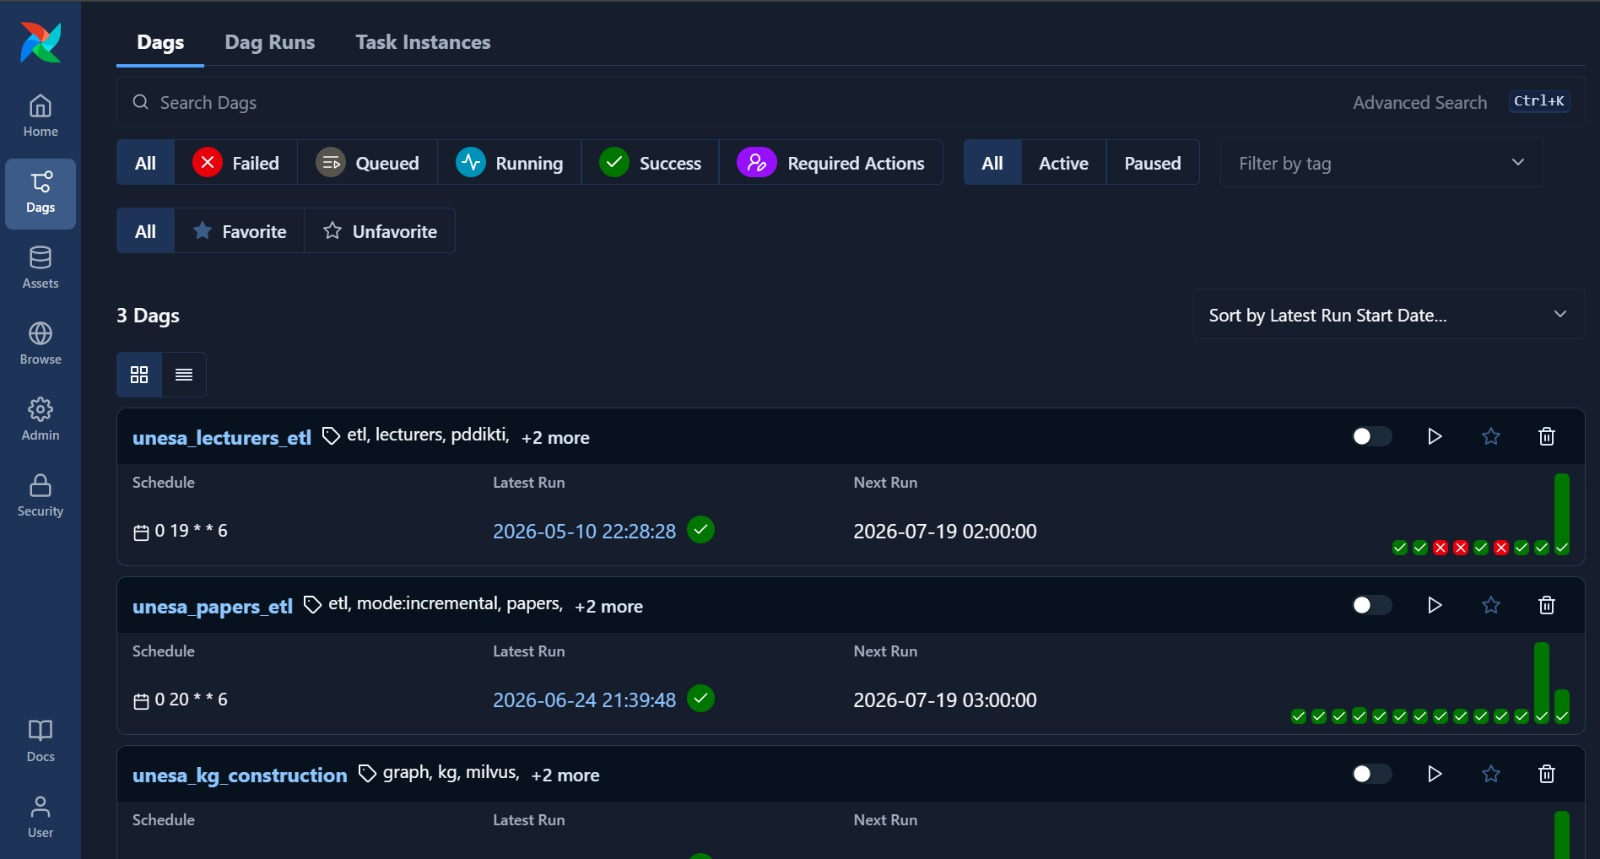
\includegraphics[width=0.98\textwidth]{Figure/airflow_dags.png}
        \caption{Halaman utama Airflow produksi dengan daftar DAG aktif}
        \label{fig:airflow-dashboard}
    \end{figure}

    \begin{figure}[htbp]
        \centering
        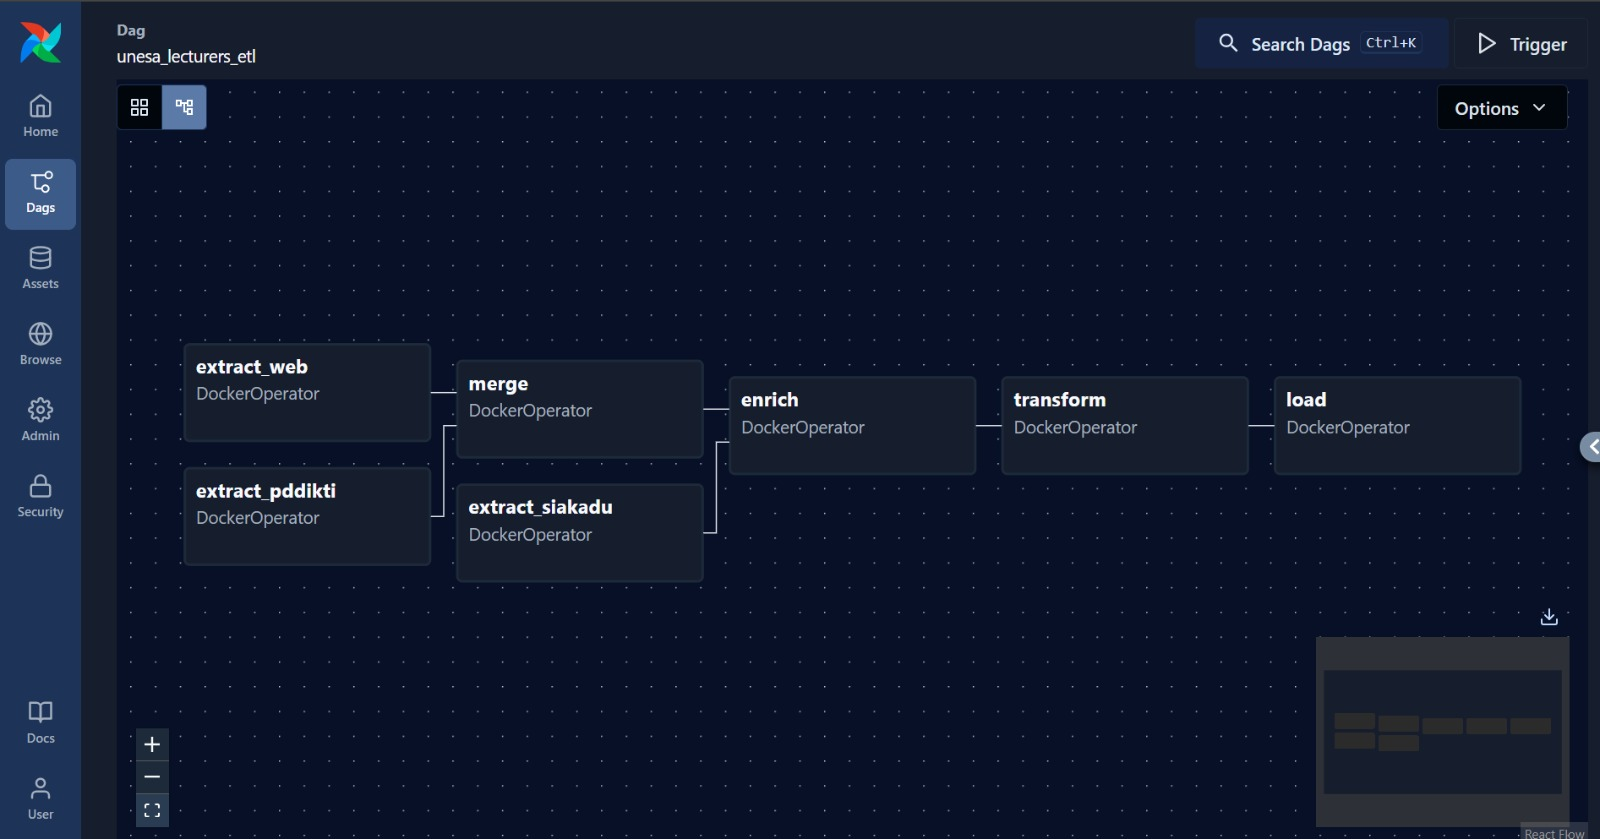
\includegraphics[width=0.98\textwidth]{Figure/airflow_lecturers_dag.png}
        \caption{Graf dependensi tugas DAG profil dosen (\texttt{unesa\_lecturers\_etl})}
        \label{fig:airflow-lecturers-dag}
    \end{figure}

    \begin{figure}[htbp]
        \centering
        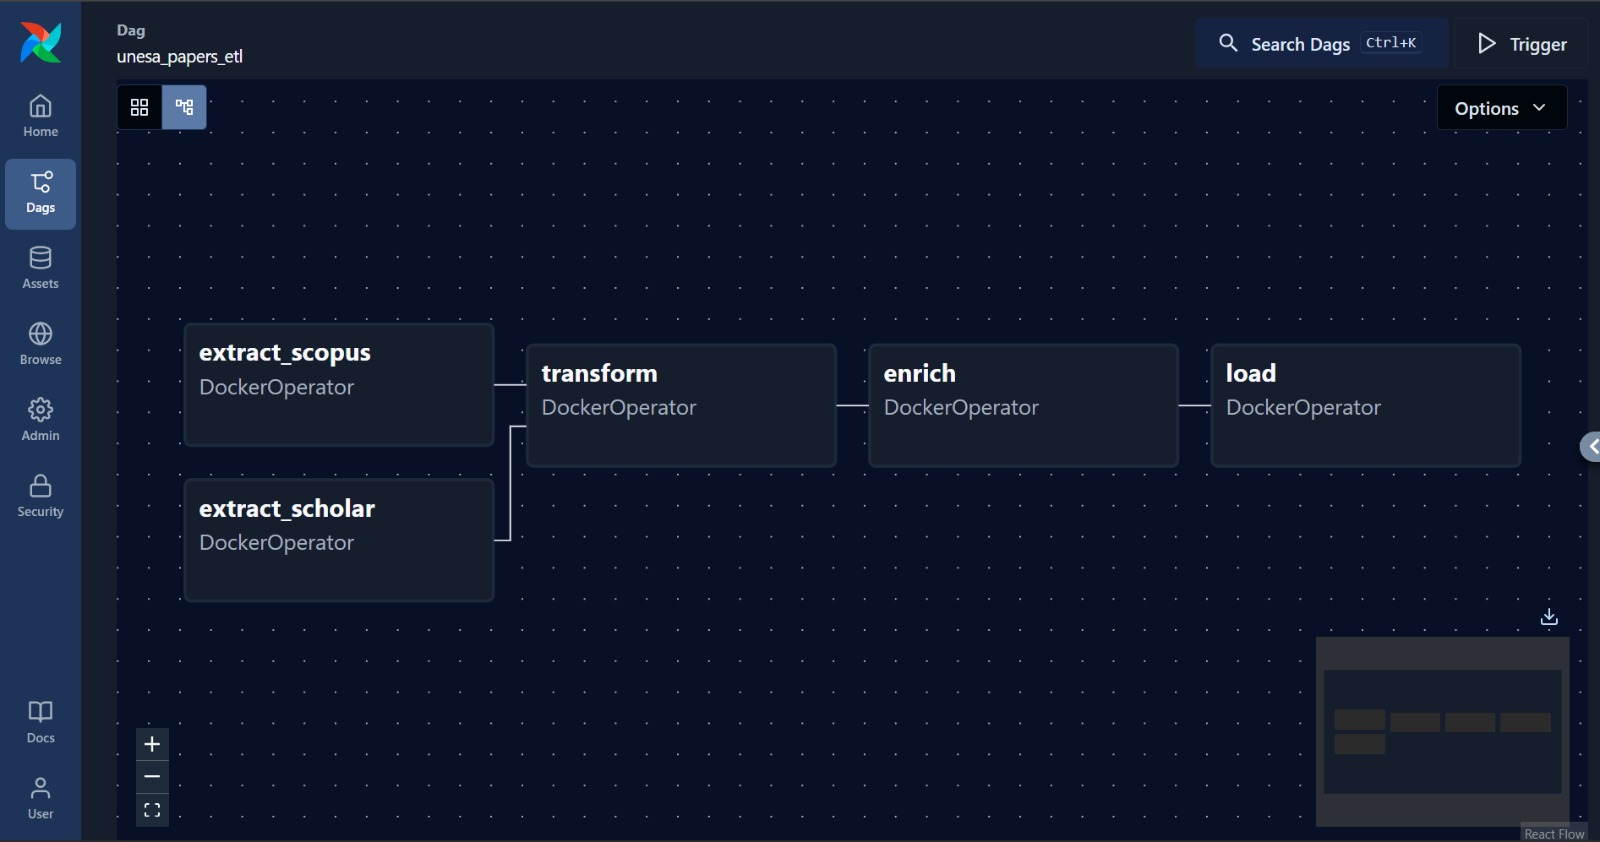
\includegraphics[width=0.98\textwidth]{Figure/airflow_papers_dag.png}
        \caption{Graf dependensi tugas DAG publikasi ilmiah (\texttt{unesa\_papers\_etl})}
        \label{fig:airflow-papers-dag}
    \end{figure}

    Dari aspek resiliensi, penarikan data Google Scholar yang rentan terhadap pemblokiran IP melalui mekanisme \textit{automatic retry} yang dikombinasikan dengan rotasi proxy residensial BrightData Web Unlocker. Selain itu, penerapan \textit{checkpoint recovery} terbukti menghemat penggunaan kuota API Scopus dan OpenAlex hingga 85\% saat melakukan menjalankan task yang gagal, karena sistem melanjutkan proses dari titik terakhir yang berhasil disimpan.

\end{sloppypar}

\section{Kesimpulan}
\begin{sloppypar}
    Rancang bangun pipeline ETL akademik menggunakan Apache Airflow yang diterapkan pada server AWS EC2 terbukti efektif dalam mengintegrasikan data profil dosen dan publikasi ilmiah di Universitas Negeri Surabaya secara otomatis dan berkala. Seluruh komponen sistem dijalankan dalam lingkungan kontainer Docker untuk menjaga konsistensi dan kemudahan pengelolaan. Pipeline berhasil menyinkronkan 128 profil dosen aktif rumpun Informatika dan Komputer serta 6.194 publikasi ilmiah unik dari enam sumber data (PDDIKTI, SIAKADU, SimCV, Sinta, Scopus, dan Google Scholar).

    Penggabungan data berhasil menyelesaikan masalah duplikasi profil dosen dan tumpang tindih data publikasi antar-platform secara akurat. Penjadwalan bertahap secara bulanan, pencatatan titik pemulihan (\textit{checkpointing}), serta penggunaan rotasi proxy residensial meningkatkan ketahanan sistem terhadap pemblokiran IP dan menghemat penggunaan kuota layanan eksternal hingga 85\% saat terjadi gangguan jaringan.

    Penelitian selanjutnya disarankan untuk memperluas kemampuan pemrosesan secara terdistribusi serta menambahkan dasbor pemantauan kesehatan pipeline secara langsung untuk memudahkan pengelolaan oleh administrator perguruan tinggi.
\end{sloppypar}

\begin{acknowledgement}[title={Ucapan Terima Kasih}]
    Penulis menyampaikan terima kasih kepada Program Studi S1 Sains Data, Universitas Negeri Surabaya, serta semua pihak yang telah memberikan dukungan dalam penyelesaian penelitian ini. Ucapan terima kasih secara khusus disampaikan kepada Ibnu Febry K., S.Kom., M.Sc., Ph.D. dan Hasanuddin Al-Habib, M.Si. selaku pembimbing, atas arahan, pendampingan, dan bimbingan yang diberikan selama proses penyusunan tugas akhir ini.
\end{acknowledgement}

\bibliographystyle{apalike-id}
\bibliography{biblio}

\end{document}